\section{在凸可行域内更新}
\label{sec:opt-con-feasible-updates}

从这一节起转向求解。最直接的想法是让每个迭代点都可行：只要可行域$C$是凸集，并且某个与$C$有关的小子问题容易求解，就可以在每一步把梯度信息转换成一个仍在$C$中的新点。本节对同一类问题——$f$在闭凸集$C$上光滑——比较三种做法。它们的区别只在于每步解哪一种子问题：投影梯度法解一个欧氏距离子问题，条件梯度法解一个线性子问题，镜像下降法把欧氏距离换成由参考函数确定的散度。

\subsection{投影梯度法}
\label{sec:opt-con-projected-gradient}

\paragraph{从梯度步到投影}
第~\ref{chap:opt-nonsmooth}章把投影建立为闭凸集指示函数的邻近映射：对非空闭凸集$C$，$\Pi_C(\bm z)=\argmin_{\bm x\in C}\lVert\bm x-\bm z\rVert_2$存在唯一，由式~\eqref{eq:opt-con-projection-vi}刻画，并且非扩张，即$\lVert\Pi_C(\bm z)-\Pi_C(\bm z')\rVert_2\leq\lVert\bm z-\bm z'\rVert_2$。\term{投影梯度法}（projected gradient method）把这一运算接在普通梯度步之后。在当前点$\bm x^{(t)}$处用线性模型加距离项近似目标，并只在$C$中最小化：
\[
  \bm x^{(t+1)}=\argmin_{\bm x\in C}\Bigl\{\langle\nabla f(\bm x^{(t)}),\bm x-\bm x^{(t)}\rangle+\frac1{2\eta}\lVert\bm x-\bm x^{(t)}\rVert_2^2\Bigr\}
  =\Pi_C\bigl(\bm x^{(t)}-\eta\nabla f(\bm x^{(t)})\bigr),
\]
第二个等号由配方得到。这正是第~\ref{chap:opt-nonsmooth}章邻近梯度法在非光滑项取$\iota_C$时的形式。

\begin{algorithm}[投影梯度法]
\label{alg:opt-con-projected-gradient}
\begin{algorithmic}[1]
\Require 可行初值$\bm x^{(0)}\in C$，步长$\eta>0$（已知$L$时取$\eta\leq1/L$），容差$\epsilon$
\Ensure 可行点$\bm x^{(t)}$
\For{$t=0,1,2,\dots$}
  \State 计算梯度$\nabla f(\bm x^{(t)})$，形成中心$\bm z=\bm x^{(t)}-\eta\nabla f(\bm x^{(t)})$
  \State 求投影$\bm x^{(t+1)}=\Pi_C(\bm z)$
  \If{$\lVert\bm x^{(t)}-\bm x^{(t+1)}\rVert_2/\eta\leq\epsilon$}
    \State 返回$\bm x^{(t+1)}$
  \EndIf
\EndFor
\end{algorithmic}
\end{algorithm}

每轮的代价是一次梯度计算加一次投影。$L$未知时可以回溯：把$\eta$减半直到$f(\bm x^{(t+1)})\leq f(\bm x^{(t)})+\langle\nabla f(\bm x^{(t)}),\bm x^{(t+1)}-\bm x^{(t)}\rangle+\frac1{2\eta}\lVert\bm x^{(t+1)}-\bm x^{(t)}\rVert_2^2$，每次试探都要重新投影。

\paragraph{具体集合上的投影}
投影的数学性质是一般的，计算却依赖集合。盒约束$C=\{\bm l\leq\bm x\leq\bm u\}$可以逐坐标截断：$\Pi_C(\bm z)_k=\min\{u_k,\max\{l_k,z_k\}\}$，代价$O(d)$；例如$[0,1]^2$上$\bm z=(1.5,-0.3)^\top$的投影是$(1,0)^\top$。欧氏球$\{\lVert\bm x\rVert_2\leq R\}$的投影是$\bm z\cdot\min\{1,R/\lVert\bm z\rVert_2\}$。概率单纯形$\Delta=\{\bm x\geq\bm0,\ \sum_kx_k=1\}$的坐标被总和约束耦合，不能逐坐标截断。对$\min\frac12\lVert\bm p-\bm z\rVert_2^2$、$\sum_kp_k=1$、$\bm p\geq\bm0$写KKT条件：$p_k-z_k+\nu-\mu_k=0$，$\mu_k\geq0$，$\mu_kp_k=0$。$p_k>0$时$\mu_k=0$、$p_k=z_k-\nu$；$p_k=0$时$z_k-\nu=-\mu_k\leq0$。两种情况合写为
\[
  p_k=\max\{z_k-\nu,0\},
\]
所有坐标共用一个阈值$\nu$，它由$\sum_k\max\{z_k-\nu,0\}=1$确定。左端关于$\nu$连续单调递减，把$\bm z$从大到小排序后逐个尝试正坐标的个数即可求出，代价$O(d\log d)$。例如$\bm z=(0.8,0.6,-0.1)^\top$：假设前两个坐标为正，$\nu=(0.8+0.6-1)/2=0.2$，检验$0.6-0.2>0$、$-0.1-0.2<0$，假设成立，投影为$(0.6,0.4,0)^\top$。一般凸集的投影本身可能是一个需要迭代求解的优化问题。

\paragraph{停止残差与收敛}
由式~\eqref{eq:opt-con-projection-vi}，$\bm x=\Pi_C(\bm x-\eta\nabla f(\bm x))$当且仅当$\langle\bm x-\eta\nabla f(\bm x)-\bm x,\bm y-\bm x\rangle\leq0$对所有$\bm y\in C$成立，即$\bm x$满足变分不等式~\eqref{eq:opt-con-vi}。所以投影梯度映射
\[
  \bm G_\eta(\bm x)=\frac{\bm x-\Pi_C(\bm x-\eta\nabla f(\bm x))}{\eta}
\]
为零恰好刻画一阶条件，算法~\ref{alg:opt-con-projected-gradient}用它的范数作停止量。它在无约束时退化为$\nabla f(\bm x)$。第~\ref{chap:opt-nonsmooth}章对邻近梯度法的分析在这里直接适用：$f$在$C$上凸且$L$光滑、最小点存在、$\eta\leq1/L$时，$f(\bm x^{(T)})-f^\star\leq\lVert\bm x^{(0)}-\bm x^\star\rVert_2^2/(2\eta T)$；若$f$还$\mu$强凸，到最小点的距离按$1-\eta\mu$的比率线性收缩。$f$非凸时，小的$\lVert\bm G_\eta\rVert_2$只说明接近一个满足一阶条件的点。

图~\ref{fig:opt-con-pg-fw}(a)在三角形$\{\bm x\geq\bm0,\ x_1+x_2\leq2\}$上最小化$f(\bm x)=\frac12((x_1-2.5)^2+4(x_2-1)^2)$，$L=4$。无约束最小点$(2.5,1)^\top$在三角形外，约束最优点$(1.3,0.7)^\top$在斜边上，预算乘子为$1.2$，$f^\star=0.9$。从$\bm0$出发取$\eta=1/4$：梯度为$(-2.5,-4)^\top$，梯度步到达$(0.625,1)^\top$，已在三角形内，投影不起作用；下一步的梯度步越过斜边，被投影拉回斜边，此后迭代沿斜边逼近最优点，依次为$(1.047,0.953)^\top$、$(1.205,0.795)^\top$、$(1.264,0.736)^\top$。目标是强凸的，图(b)中目标差按几何级数下降。

\paragraph{预条件必须匹配投影}
若用固定的正定矩阵$\bm M$作预条件，梯度步变为$\bm x-\eta\bm M\nabla f(\bm x)$，投影也必须换成在范数$\lVert\bm v\rVert_{\bm M^{-1}}^2=\bm v^\top\bm M^{-1}\bm v$下的最近点：
\[
  \bm x^{+}=\argmin_{\bm y\in C}\ \bigl\lVert\bm y-(\bm x-\eta\bm M\nabla f(\bm x))\bigr\rVert_{\bm M^{-1}}^2.
\]
这样，固定点条件中的$\bm M^{-1}\bm M$相互抵消，仍是原来的变分不等式。若仍用欧氏投影，固定点满足的是$\langle\bm M\nabla f(\bm x),\bm y-\bm x\rangle\geq0$，一般与原条件不同。等式二次例给出一个具体反例：取$\bm M=\operatorname{diag}(1,4)$，在约束直线上$\bm M\nabla f=(x_1,16x_2)^\top$，欧氏投影的固定点要求它与直线方向$(1,-1)^\top$正交，得到$x_1=16x_2$，即$(16/17,1/17)^\top$，而真正的最优点是$(4/5,1/5)^\top$。对角$\bm M$加盒约束时加权投影仍可逐坐标计算；对单纯形或一般耦合的$\bm M$，加权投影是一个新的子问题，代价不能按欧氏投影计算。

\paragraph{近似投影}
投影若由内层迭代求出，输出与真投影之差$\zeta_t$会带来两类后果。其一，输出可能略微不可行，必须单独检查约束残差，不能把“投影子问题的距离误差小”当作可行。其二，误差会沿迭代传播：投影非扩张，若精确的投影梯度映射在凸、$L$光滑且$\eta\leq2/L$时把距离收缩不增，则到最优点的距离满足$\delta_{t+1}\leq\delta_t+\zeta_t$，强凸时可改进为$\delta_{t+1}\leq(1-\eta\mu)\delta_t+\zeta_t$，误差最终停留在$\zeta/(\eta\mu)$量级。停止量$\lVert\bm G_\eta\rVert_2$里的误差被放大为$\zeta_t/\eta$，步长很小时尤其明显。投影的存在唯一与非扩张、具体集合上投影怎么算、外层迭代收敛多快，是三项不同的职责。

\subsection{条件梯度法}
\label{sec:opt-con-frank-wolfe}

\paragraph{用线性子问题代替投影}
对某些集合，求投影很贵，但在集合上最小化一个线性函数很便宜。例如在迹不超过$\tau$的半正定矩阵集合上，投影需要完整的特征分解，而最小化线性函数只需要一个极端特征向量。下面的方法利用这一点：把目标在当前点线性化，在$C$上求线性模型的最小点，再沿当前点与该点的连线移动一段。$C$紧时线性子问题总有解，新点是两个可行点的凸组合，自动可行。这就是\term{条件梯度法}（conditional gradient method），由Frank与Wolfe提出\scite{frank1956algorithm}，也称Frank--Wolfe法。

\begin{algorithm}[条件梯度法]
\label{alg:opt-con-frank-wolfe}
\begin{algorithmic}[1]
\Require 非空紧凸集$C$上的线性最小化程序，可行初值$\bm x^{(0)}\in C$，容差$\epsilon$
\Ensure 可行点$\bm x^{(t)}$及条件梯度间隙
\For{$t=0,1,2,\dots$}
  \State 计算梯度，解线性子问题$\bm s^{(t)}\in\argmin_{\bm s\in C}\langle\nabla f(\bm x^{(t)}),\bm s\rangle$
  \State 计算间隙$\gamma_t=\langle\nabla f(\bm x^{(t)}),\bm x^{(t)}-\bm s^{(t)}\rangle$；若$\gamma_t\leq\epsilon$，返回$\bm x^{(t)}$
  \State 取步长$\alpha_t=2/(t+2)$（或在线段上作一维线搜索），更新$\bm x^{(t+1)}=\bm x^{(t)}+\alpha_t(\bm s^{(t)}-\bm x^{(t)})$
\EndFor
\end{algorithmic}
\end{algorithm}

\paragraph{线性子问题的稀疏与低秩解}
线性函数在紧凸集上的最小值总能在极点处取到，所以线性子问题的解往往很“简单”。在单纯形上，它是梯度最小坐标对应的顶点$\bm e_k$；从一个顶点出发，$t$步以后迭代点至多是$t+1$个顶点的凸组合，至多有$t+1$个非零坐标。在$\{\bm S\succeq\bm0,\ \operatorname{tr}\bm S\leq\tau\}$上，记$\bm W=\nabla f(\bm X)$的最小特征值为$\lambda_{\min}$、对应单位特征向量为$\bm v$。对该集合中任意$\bm S$，用$\bm S$的谱分解$\bm S=\sum_k\sigma_k\bm u_k\bm u_k^\top$得$\langle\bm W,\bm S\rangle=\sum_k\sigma_k\bm u_k^\top\bm W\bm u_k\geq\lambda_{\min}\operatorname{tr}\bm S\geq\tau\min\{\lambda_{\min},0\}$，所以$\lambda_{\min}<0$时线性子问题的解是秩一矩阵$\tau\bm v\bm v^\top$，否则是$\bm0$。迭代$t$步后，矩阵的秩至多为$t$，求解过程只需存储这些秩一因子。

\paragraph{条件梯度间隙与收敛速度}
算法中的$\gamma_t$同时是一份证书。若$f$凸，由一阶支撑下界，对最优点$\bm x^\star$，
\[
  f(\bm x^{(t)})-f^\star\leq\langle\nabla f(\bm x^{(t)}),\bm x^{(t)}-\bm x^\star\rangle\leq\max_{\bm s\in C}\langle\nabla f(\bm x^{(t)}),\bm x^{(t)}-\bm s\rangle=\gamma_t,
\]
因此不知道$f^\star$也能确定目标差的上界；$\gamma_t=0$恰好是变分不等式~\eqref{eq:opt-con-vi}。

\begin{theorem}[条件梯度法的收敛速度]
\label{thm:opt-con-frank-wolfe}
设$C$非空紧凸，直径为$D=\max_{\bm x,\bm y\in C}\lVert\bm x-\bm y\rVert_2$，$f$在$C$的开邻域上凸且$L$光滑。取$\alpha_t=2/(t+2)$，则对$t\geq1$，$f(\bm x^{(t)})-f^\star\leq2LD^2/(t+2)$。
\end{theorem}

\begin{proof}
记$e_t=f(\bm x^{(t)})-f^\star$。由$L$光滑的二次上界，并利用$\lVert\bm s^{(t)}-\bm x^{(t)}\rVert_2\leq D$与上式$\langle\nabla f(\bm x^{(t)}),\bm s^{(t)}-\bm x^{(t)}\rangle=-\gamma_t\leq-e_t$，
\[
  e_{t+1}\leq e_t+\alpha_t\langle\nabla f(\bm x^{(t)}),\bm s^{(t)}-\bm x^{(t)}\rangle+\frac{L\alpha_t^2D^2}{2}\leq(1-\alpha_t)e_t+\frac{L\alpha_t^2D^2}{2}.
\]
$t=0$时$\alpha_0=1$，得$e_1\leq LD^2/2\leq2LD^2/3$。若$e_t\leq2LD^2/(t+2)$，代入$\alpha_t=2/(t+2)$，
\[
  e_{t+1}\leq\frac{t}{t+2}\cdot\frac{2LD^2}{t+2}+\frac{2LD^2}{(t+2)^2}=\frac{2LD^2(t+1)}{(t+2)^2}\leq\frac{2LD^2}{t+3},
\]
最后一步用了$(t+1)(t+3)\leq(t+2)^2$。归纳即得。
\end{proof}

图~\ref{fig:opt-con-pg-fw}对比同一问题上的两种方法。条件梯度法从$\bm0$出发，第一步的线性子问题选中顶点$(0,2)^\top$（梯度$(-2.5,-4)^\top$与该顶点内积最小），步长$\alpha_0=1$，直接跳到该顶点；此后线性子问题在顶点$(2,0)^\top$与$(0,2)^\top$之间交替，迭代点沿斜边来回振荡逼近最优点。最优点位于斜边内部而不在顶点上，这种“之”字形使目标差只按$O(1/t)$减小并伴随振荡：$100$步时目标差约为$7\times10^{-5}$，而投影梯度法$15$步内已达到$10^{-12}$。条件梯度间隙也在振荡，所以实际停止时常记录迄今最小的间隙。

\begin{figure*}[!htbp]
  \centering
  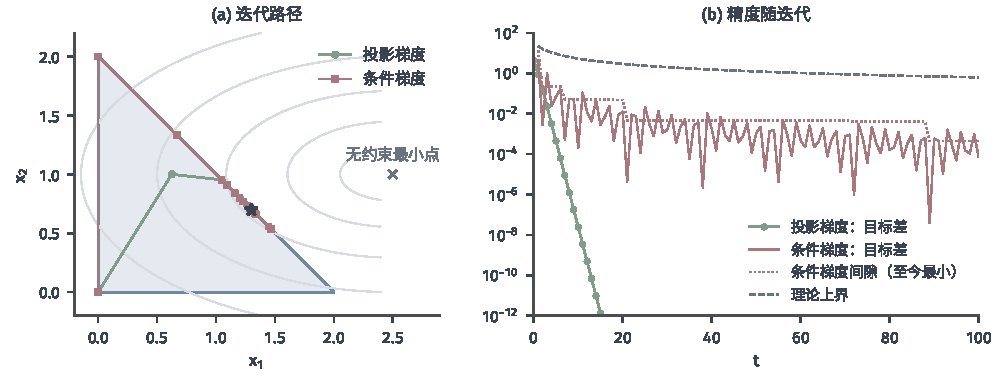
\includegraphics[width=169mm]{figures/03-optimization-evolution-and-signals/01-optimization/matplotlib/c5-pg-fw/figure.pdf}
  \caption{三角形$\{\bm x\geq\bm0,\ x_1+x_2\leq2\}$上最小化$\frac12((x_1-2.5)^2+4(x_2-1)^2)$，起点$\bm0$。(a) 灰色椭圆为等值线，五角星为最优点$(1.3,0.7)^\top$；绿色为投影梯度法（$\eta=1/4$），红色为条件梯度法（$\alpha_t=2/(t+2)$），后者在两个顶点之间交替选点，沿斜边振荡。(b) 对数纵轴上的目标差：投影梯度法线性收敛；条件梯度法的目标差振荡下降，红色点线为迄今最小的条件梯度间隙，灰色虚线为定理~\ref{thm:opt-con-frank-wolfe}的上界$2LD^2/(t+2)$，$L=4$，$D=2\sqrt2$。}
  \label{fig:opt-con-pg-fw}
\end{figure*}

两种方法应在同一精度口径下比较每轮成本。单纯形或盒约束上投影与线性子问题都很便宜，投影梯度法通常更快。迹约束的半正定集合上，投影需要$O(k^3)$的完整特征分解，而线性子问题只需一个极端特征向量，可用Lanczos类迭代以若干次矩阵向量积近似求得；条件梯度法因此常被用于低秩矩阵问题。代价是收敛较慢：最优点落在集合边界的面内部时，要获得高精度需要很多次迭代。

\subsection{镜像下降法}
\label{sec:opt-con-mirror-descent}

\paragraph{欧氏距离不总是合适的尺度}
在概率单纯形上，从$x_k=0.01$变到$0.02$与从$0.5$变到$0.51$的欧氏距离相同，但前者让这个坐标翻了一倍。投影梯度法用欧氏距离衡量步子，会在一步之内把小坐标截成零（图~\ref{fig:opt-con-mirror-simplex}中第三个坐标在第3步恰好变为零），而后续步骤只能从边界上重新开始。\term{镜像下降法}（mirror descent）把投影梯度法中的$\frac12\lVert\bm x-\bm x^{(t)}\rVert_2^2$换成一个更贴合集合几何的“距离”。

\begin{definition}[Bregman散度]
\label{def:opt-con-bregman}
设$\varphi$是在开凸集$\operatorname{int}\operatorname{dom}\varphi$上可微的严格凸函数，称
\[
  D_\varphi(\bm x,\bm y)=\varphi(\bm x)-\varphi(\bm y)-\langle\nabla\varphi(\bm y),\bm x-\bm y\rangle,\qquad\bm x\in\operatorname{dom}\varphi,\ \bm y\in\operatorname{int}\operatorname{dom}\varphi
\]
为$\varphi$生成的\term{Bregman散度}（Bregman divergence），$\varphi$称为参考函数。
\end{definition}

$D_\varphi(\bm x,\bm y)$是$\varphi$在$\bm x$处的值超出它在$\bm y$处切平面的部分；由严格凸性，它非负，且仅在$\bm x=\bm y$时为零。它一般不对称，也不满足三角不等式，所以不是度量。取$\varphi(\bm x)=\frac12\lVert\bm x\rVert_2^2$得$D_\varphi(\bm x,\bm y)=\frac12\lVert\bm x-\bm y\rVert_2^2$。取负熵$\varphi(\bm x)=\sum_kx_k\log x_k$（定义在$\bm x\geq\bm0$上，约定$0\log0=0$），对单纯形中的$\bm x$与正向量$\bm y\in\Delta$，$D_\varphi(\bm x,\bm y)=\sum_kx_k\log(x_k/y_k)$。例如$\bm x=(1/2,1/2)$、$\bm y=(1/4,3/4)$时$D_\varphi(\bm x,\bm y)=\frac12\log2+\frac12\log\frac23\approx0.144$，而$D_\varphi(\bm y,\bm x)=\frac14\log\frac12+\frac34\log\frac32\approx0.131$，两者不同。

\paragraph{镜像下降的更新}
把散度放进线性化子问题，镜像下降的一步为
\begin{equation}
\label{eq:opt-con-mirror-step}
  \bm x^{(t+1)}\in\argmin_{\bm x\in C\cap\operatorname{dom}\varphi}\Bigl\{\eta\langle\nabla f(\bm x^{(t)}),\bm x\rangle+D_\varphi(\bm x,\bm x^{(t)})\Bigr\}.
\end{equation}
它要求$\bm x^{(t)}$在$\varphi$的可微域内部，否则$D_\varphi(\cdot,\bm x^{(t)})$无定义；严格凸只保证子问题至多一个解，解的存在、以及解是否仍在可微域内部（下一步能否继续），要针对具体的$\varphi$和$C$另外核查。欧氏参考函数下，式~\eqref{eq:opt-con-mirror-step}就是投影梯度步。

在单纯形上取负熵，并从正权重出发。式~\eqref{eq:opt-con-mirror-step}的目标为$\sum_k(\eta g_kx_k+x_k\log(x_k/x_k^{(t)}))$，其中$\bm g=\nabla f(\bm x^{(t)})$（单纯形上$\sum_kx_k=\sum_kx_k^{(t)}$，散度中的线性项抵消）。对等式$\sum_kx_k=1$引入乘子$\nu$，令偏导为零：$\eta g_k+\log(x_k/x_k^{(t)})+1+\nu=0$，于是
\begin{equation}
\label{eq:opt-con-exponential-weights}
  x_k^{(t+1)}=\frac{x_k^{(t)}\exp(-\eta g_k)}{\sum_lx_l^{(t)}\exp(-\eta g_l)}.
\end{equation}
这是乘以指数因子再归一化的\emph{指数权重更新}。梯度有限时指数因子严格为正，正权重永远保持为正，非负约束从不活跃，所以忽略它们的拉格朗日计算是合法的；$\log$在边界处的无界导数自动把迭代挡在内部。

图~\ref{fig:opt-con-mirror-simplex}在单纯形上最小化$f(\bm x)=\frac12\lVert\bm x-\bm c\rVert_2^2$，$\bm c=(0.8,0.6,-0.1)^\top$，最优点是前面算过的投影$(0.6,0.4,0)^\top$，从$\bm x^{(0)}=(0.15,0.15,0.7)^\top$出发。镜像下降取$\eta=1$：$\bm g=\bm x^{(0)}-\bm c=(-0.65,-0.45,0.8)^\top$，未归一化的权重为$0.15e^{0.65}\approx0.2873$、$0.15e^{0.45}\approx0.2352$、$0.7e^{-0.8}\approx0.3145$，归一化得$\bm x^{(1)}\approx(0.343,0.281,0.376)^\top$。投影梯度取$\eta=0.5$：中心$\bm x^{(0)}-0.5\bm g=(0.475,0.375,0.3)^\top$，坐标和为$1.15$，共同阈值$0.05$，得$\bm x^{(1)}=(0.425,0.325,0.25)^\top$。两条路径都走向最优点，但投影梯度法在第3步把第三个坐标截为零后沿边界移动，镜像下降的第三个坐标始终为正，按指数速度趋于零。

\begin{figure*}[!htbp]
  \centering
  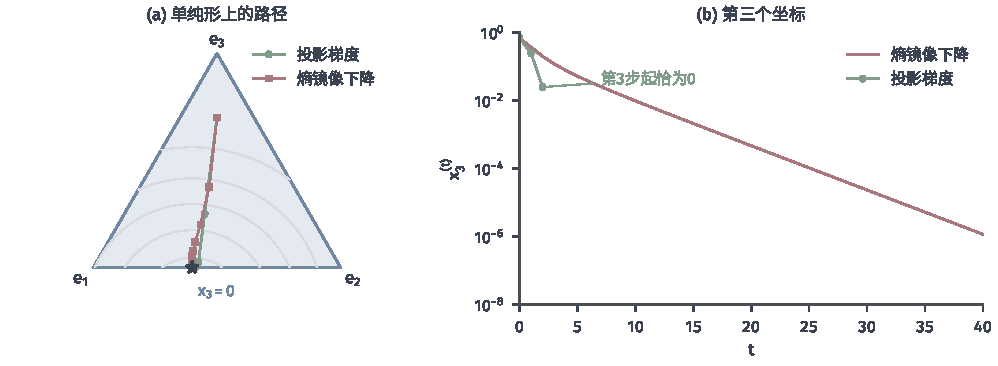
\includegraphics[width=169mm]{figures/03-optimization-evolution-and-signals/01-optimization/matplotlib/c5-mirror-simplex/figure.pdf}
  \caption{概率单纯形上最小化$\frac12\lVert\bm x-\bm c\rVert_2^2$，$\bm c=(0.8,0.6,-0.1)^\top$，起点$(0.15,0.15,0.7)^\top$。(a) 单纯形用重心坐标画成三角形，顶点$\bm e_k$对应第$k$个坐标为$1$，灰色曲线为目标等值线，五角星为最优点$(0.6,0.4,0)^\top$，位于$x_3=0$的边上。绿色为投影梯度法（$\eta=0.5$），红色为熵镜像下降（$\eta=1$）。(b) 第三个坐标随迭代的变化（对数纵轴）：投影梯度法在第3步起恰为零，镜像下降保持为正并几何下降。}
  \label{fig:opt-con-mirror-simplex}
\end{figure*}

参考函数的选择影响的不只是路径形状。对单纯形上的凸、梯度各分量有界（$\lVert\nabla f\rVert_\infty\leq G$）的问题，熵镜像下降的目标差界依赖$\sqrt{\log d}$，而欧氏投影的相应界依赖梯度的欧氏范数，可能大到$\sqrt dG$，维数高时前者显著更好\scite{beck2003mirror}。这里只建立有限维的优化机制。上面单纯形上的负熵散度就是离散分布之间的KL散度，它作为分布间散度的系统性质、相应的几何及统计解释，可参考\BookChapterRef{chap:information-theory-and-statistical-geometry}{卷四“概率分布的分析与优化”章}。
